% 第2章 文献综述

\chapter{二、文献综述}

\section{1.国内外研究现状、发展动态}

\subsection{（1）激光光源发展}

\subsubsection{染料激光的发展}

国外研究现状。染料激光是最早实现宽带连续可调谐的相干光源之一，自 20 世纪 60 年代中期问世起即成为光谱学与激光化学的主力光源。Duarte 系统梳理了高性能液体与固体窄线宽染料激光振荡器的物理机理与技术体系，指出染料分子宽荧光谱带来的调谐范围优势，与其热透镜效应、三重态吸收、光化学退化等固有限制并存\cite{ref1}；Pavlopoulos 等则从分子结构—光谱性能关联的角度归纳了激光染料的构效关系，为不同波段染料选型提供依据\cite{ref2}。

为克服液体染料的热管理与寿命问题，器件化沿两条路线推进：一条是固体化路线，Duarte 与 James 将染料掺杂聚合物—纳米颗粒复合增益介质引入可调谐固体激光器，在保持调谐能力的同时显著提升光稳定性\cite{ref3}；另一条是分布式反馈（DFB）集成路线，Oki 等利用塑料波导 DFB 结构实现长寿命、高重复频率的染料激光输出\cite{ref4}。泵浦方式也在更新，Burdukova 等报道了半导体激光直接泵浦的可调谐染料激光，摆脱传统 Nd:YAG 或准分子激光泵浦的体积与功耗约束\cite{ref5}。

将染料激光推进到燃烧诊断所需的高重复频率是近年关键进展。Pan 等构建了脉冲串染料激光系统，实现千赫兹重复频率下的高能窄带可调紫外输出，首次把染料激光的宽带调谐能力与脉冲串泵浦的高帧频优势结合起来\cite{ref6}；Mishra 等针对高重复频率脉冲染料激光长期存在的染料池热积累与流场退化问题，用 PIV 对染料池内流场进行表征，指出染料循环与池体结构是高重频下光束质量退化的主控因素\cite{ref7}。

国内研究现状。国内在染料激光本体方向公开报道相对有限，近年有代表性的工作集中在``脉冲串染料激光''这一交叉点上。Chen 等研制了 10 kHz 重复频率、高单脉冲能量的脉冲串染料激光器，系统解决了高重频条件下染料增益介质的热致波前畸变、脉冲串包络均匀性与窄线宽保持问题\cite{ref8}；与之配套，Li 等研制了 10 kHz、10 ns、13.4 mJ 的 Nd:YAG 三倍频脉冲串 MOPA 泵浦源（355 nm），为染料激光提供高重频、高能量的紫外泵浦\cite{ref9}。

\subsubsection{串脉冲（burst-mode）激光器发展}

国外研究现状。脉冲串激光的概念由 Lempert 等在 1996 年提出，其核心思想是用低占空比的短脉冲串替代连续高重频运行，在保持极高瞬时重复频率（可达 MHz）的同时把平均热负载控制在可承受范围\cite{ref10}。随后 Wu 与 Miles 建成 MHz 级高能脉冲串激光系统，并完成激波/边界层干扰的序列可视化\cite{ref11}，标志着该技术进入高速流动诊断实用阶段。

此后发展沿两条主线推进。一是窄线宽化：Thurow 等研制窄线宽 MHz 脉冲串激光器\cite{ref12}，使脉冲串光源可直接服务于需要窄线宽激发的 PLIF 测量，并迭代至第三代系统\cite{ref13}；Jiang 等提出改进的高重频脉冲串输出产生方法，显著改善脉冲串内能量一致性\cite{ref14}。二是能量与时宽扩展：Slipchenko 等实现 100 kHz、100 ms、400 J 的双波长二极管泵浦放大脉冲串激光器\cite{ref15}；Roy 等实现 100 ps 脉宽、100 J 级脉冲串输出以覆盖 kHz--MHz 诊断需求\cite{ref16}；Michael 等把千帧级、100 kHz 的平面成像带入湍流火焰\cite{ref17}；Roy 等进一步提出``三路输出''（three-legged）脉冲串激光架构，实现速度场与多个标量场的同时测量\cite{ref18}。Slipchenko 等在 2021 年燃烧学大会上对脉冲串激光诊断在反应流/非反应流中的进展作了权威综述，明确指出高重频脉冲串泵浦染料激光/OPO 是实现高速自由基成像的关键路径\cite{ref19}；Jiang 等则聚焦高超声速流动场景做了最新总结\cite{ref20}。

国内研究现状。国内以哈尔滨工业大学（陈德应、李旭东、闫仁鹏、于欣等）为主的团队已形成较完整的脉冲串激光技术链。闫仁鹏等采用 YAG/Nd:YAG/Cr$^{4+}$:YAG 复合晶体实现高重频、高峰值功率脉冲串输出\cite{ref21}；吴文韬等通过增益分布控制的侧面泵浦实现平顶光束输出的腔倒空脉冲串 MOPA 系统\cite{ref22}；近年工作进一步向高重频、窄线宽、包络整形方向发展，于欣等实现 100 kHz 窄线宽、包络均匀的脉冲串 MOPA 系统\cite{ref23}，徐浩波等在 2025 年用变反射率非稳腔进一步优化高重频脉冲串 Nd:YAG 输出\cite{ref24}。

如图 2 为脉冲串激光产生原理，图 3\cite{ref25} 为染料激光从 1963—2019 年的发展历史。从图中可以看出：单次 burst 内脉冲数量（绿色 M）持续增加，从早期几个脉冲发展到单次 burst 上百个脉冲，支持更多帧连续 PLIF 图像；脉冲串持续时间不断拉长，从 0.1 ms 发展到数 ms、最长可达 30 ms，给湍流火焰更长的高速观测窗口；重复频率（蓝色 f）与单 burst 总能量同步提升，既能做到 kHz/MHz 高频子脉冲，又保留足够高的脉冲能量，满足紫外倍频做 NO-PLIF 的能量需求。

\begin{figure}[H]
  \centering
  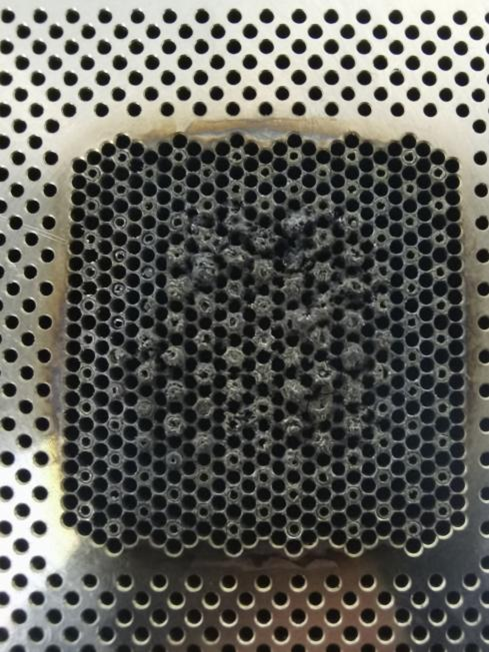
\includegraphics[width=0.75\textwidth]{figures/image2.png}
  \caption{Pulse-burst 激光产生原理}
  \label{fig:burst-principle}
\end{figure}

\begin{figure}[H]
  \centering
  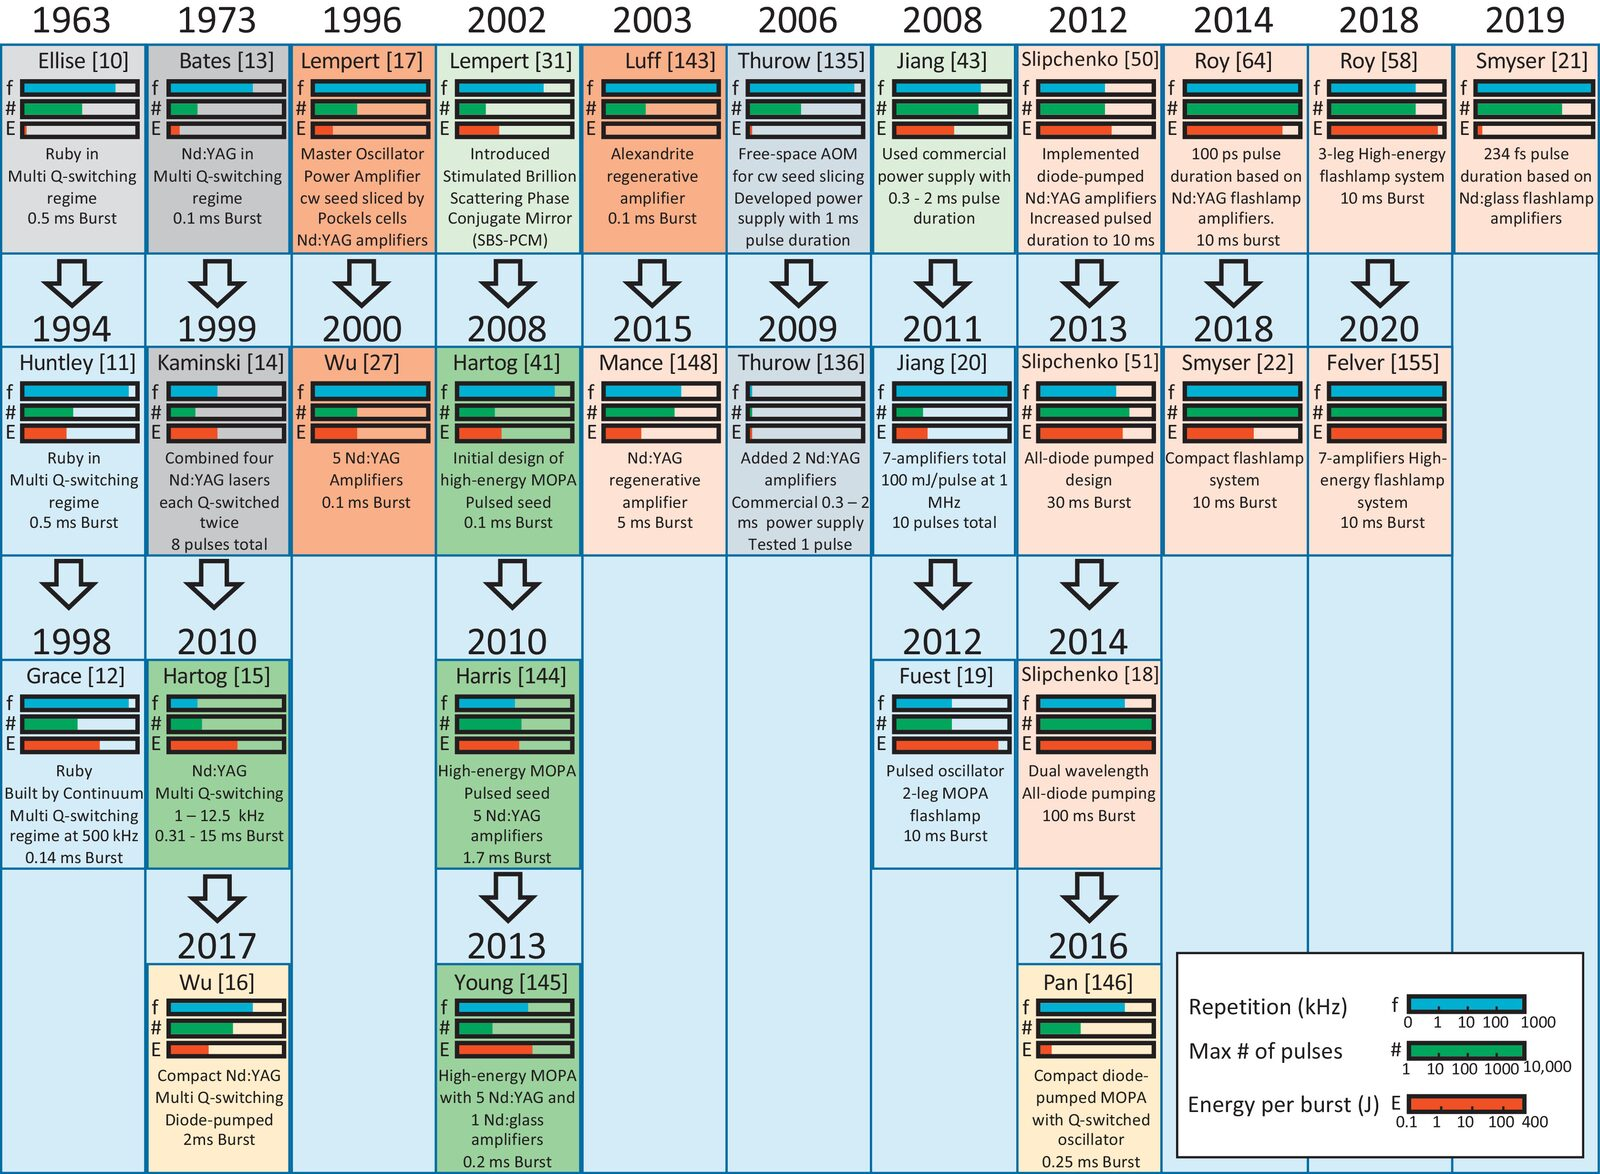
\includegraphics[width=0.85\textwidth]{figures/image3.jpeg}
  \caption{burst 染料激光发展历程}
  \label{fig:burst-history}
\end{figure}

\subsection{（2）PLIF（平面激光诱导荧光）发展}

\subsubsection{国外研究现状}

PLIF 由点测量 LIF 发展而来：Ald\'{e}n 等 1982 年用二极管阵列探测器获得大气火焰中 OH 荧光的单脉冲空间分辨图像\cite{ref26}；Allen 等随后用 CH 与 C$_2$ 的 PLIF 对碳氢—空气火焰反应区进行数字成像，标志着 PLIF 成为燃烧二维成像的主流手段\cite{ref27}。

定量化是长期难点，核心是碰撞猝灭。Tamura 等系统测定了低压碳氢火焰中 CH(A)、OH(A)、NO(A) 的碰撞猝灭规律\cite{ref28}，为荧光信号的温度与组分依赖校正提供了物理基础；此后围绕 NO(A$^2\Sigma^+$) 与 O$_2$、H$_2$O 等非反应/反应碰撞猝灭动力学的成像研究持续推进。这一物理机制决定了：PLIF 给出的是``相对荧光强度分布''，要转化为绝对浓度必须解决猝灭速率的温度—组分依赖与激发效率标定问题。

高重复频率化是 PLIF 近二十年的主旋律。Jiang 等实现 500 kHz 帧频的 NO-PLIF 成像\cite{ref29}，并在 CUBRC 48 英寸激波风洞完成 NO-PLIF 流场成像；Hammack 等在 10 kHz 下对 seeded 流场、等离子体放电与火焰中的 NO 进行 PLIF 测量\cite{ref30}；在 OH/CH$_2$O 等组分的高速成像与多参量同步方面，Wang 等实现湍流火焰中多组分同步超高速 PLIF 成像\cite{ref31}，Halls 等用脉冲串体激光诱导荧光获得燃烧中间组分的四维时空演化\cite{ref32}，Hsu 等在旋转爆震燃烧室中实现 MHz 级 OH-PLIF 成像\cite{ref33}，Hammack 等把 20 kHz CH$_2$O/OH-PLIF 与立体 PIV 同步。针对高重频 NO-PLIF 的光源瓶颈，Leonov 等对用于高重频 NO-PLIF 的光参量振荡器（OPO）进行优化设计\cite{ref34}，Rodrigues 等实现 100 kHz 高光谱分辨率 NO-PLIF 测量\cite{ref35}。

Wang 等用单台染料激光同时成像氨—氢—氮火焰中的 NO 与 NH\cite{ref36}；Chatelain 等用单台染料激光实现 NO 与 OH 的同时 PLIF\cite{ref37}；Wang 等进一步实现 NH$_3$、NH、NO 三组分的同时测量\cite{ref38}；Tang 等把 NH/NO 同步 PLIF 用于等离子体助燃氨/氢旋流火焰。这些工作证明了染料激光在 NO-PLIF 中的独特价值——宽带调谐使一台染料激光即可覆盖多个自由基的激发线，正好呼应前文``脉冲串染料激光''的发展方向，也为``一台光源、多组分同步成像''提供了直接的技术范式。

\subsubsection{国内研究现状}

国内 PLIF 研究起步稍晚但发展迅速。陈爽等提出火焰中瞬时二维 OH-PLIF 测温的标定方法\cite{ref39}；刘训臣等用双波长切换的脉冲串激光实现单相机 20 kHz 双色甲醛 PLIF 测温\cite{ref40}；在超燃冲压方向，王林森等用 acetone-PLIF 研究燃烧室燃料/空气掺混特性，万明罡等提出在强火焰自发光背景下实现瞬时 CH$_2$O-PLIF 成像的策略，汪洪波等用高速相机与双组分 PLIF 同步技术可视化超声速燃烧\cite{ref41}；在旋流燃烧方向，尹盛铭等对双级径向旋流燃烧室的火焰形态转变进行了激光诊断研究。

\section{（3）现有研究的不足与本课题切入点}

综合上述文献，现有研究仍存在以下不足，构成本课题的切入点：

（1）多组分 TDLAS 与自由基 PLIF 多为独立系统，缺乏同一标准场下的交叉校验与一体化标定；

（2）中红外 QCL 与 burst 染料激光共用时序、触发与数据采集的同步机制尚不成熟；

（3）burst 染料激光在高电感/高频工况下的稳定性（能量抖动、线宽展宽、波长漂移）控制缺乏系统研究。

发展趋势：由单组分向多组分、由近红外向中红外、由离线标定向原位在线、由单点向多线/断层成像演进。本课题正是在这一趋势下，围绕``线定量 + 场成像''一体化诊断展开。

\section{所阅文献的查阅范围及手段；参考资料}

参考资料（所阅主要文献）：

\printbibliography[heading=none]
